% !TEX root = ~/OpenFOAM/antoniopucciarelli-9/run/LABS/thermochemical_CFD/main.tex

\section{Reacting flows - $\mathtt{Lab07}$} \label{sec:lab07}
    
    \renewcommand{\thepage}{\arabic{page}}
    \setcounter{page}{\thelastPage}
    
    This section treats the numerical modeling of chemical reactions. Reactions are treated as well as the spray modeling and the wall-film surface modeling, they are seen as an \textbf{additional layer} to the \verb|FVM| problem. This additional modeling layer has to be blended into the \textit{main} flow solution as it happened with lagrangian spray modeling and wall-film modeling.
The important concepts related to combustion theory and modeling are explained in~\ref{app:app4}.
%    \subsection{Reactions}
%    Before starting modeling reactions it is necessary to know the species inside the system, the possible reactions that can happen and all the parameters related to transport and diffusion of these species into the system. All these properties are mainly taken from experiments or they come from chemistry modeling (for the more complicated species). 
    
%    \subsubsection{Govering equations}
%    The main changes in the governing equation are made on the continuity equation. The continuity equation expresses the conservation of mass in the system. Because the presence of reactions, it is needed to track the species' evolution in the system. The continuity equations for each species are written as:
%    \begin{equation}
%        \frac{\partial \rho Y_i}{\partial t} + \boldsymbol{\nabla} \cdot \big( \rho \boldsymbol{u} \ Y_i  \big) = \boldsymbol{\nabla} \cdot \big( \rho \boldsymbol{v}_i \ Y_i \big) + \dot\omega_i
%    \end{equation}
%    Where $Y_i$ is the mass fraction of \textit{ith} species, $\boldsymbol{v}_i$ is the \textit{ith} species diffusion velocity\footnote{$\sum_i \boldsymbol{\nabla} \cdot \big( \rho Y_i \boldsymbol{v}_i \big) = 0$, where $\boldsymbol{v}_i$ is the species velocity fluctuation, $\sum_i Y_i = 1$ and $\boldsymbol{\nabla} \cdot \big( \rho \boldsymbol{u} \big) = 0$. \newline $\sum_i \boldsymbol{\nabla} \cdot \big[ Y_i \rho \big(\boldsymbol{u} + \boldsymbol{v}_i \big) \big] = \sum_i \boldsymbol{\nabla} \cdot \big( Y_i \rho \boldsymbol{u} \big) + \sum_i \boldsymbol{\nabla} \cdot \big( Y_i \rho \boldsymbol{v}_i \big) = \boldsymbol{\nabla} \cdot \big( \rho \boldsymbol{u} \sum_i Y_i \big) + \sum_i \boldsymbol{\nabla} \cdot \big( Y_i \rho \boldsymbol{v}_i \big) = 0$.} and $\dot\omega_i$ is the \textit{ith} species production due to reactions\footnote{$\sum_i \dot\omega_i = 0$ because the reaction process does not create mass, it just \textit{moves} atoms in order to create new species, conserving mass.}. As result, $\boldsymbol{v}_i$ are new degree of freedom into the system, so it is necessary to find equations that allow to treat them. The complete equation for the $\boldsymbol{v}_i$ computation is very hard to solve\footnote{$\boldsymbol{v}_p$ equation: $\boldsymbol{\nabla}X_p = \sum_k \frac{X_p \ X_k}{\mathcal{D}_{p, k}}\big( \boldsymbol{v}_k - \boldsymbol{v}_p \big) + ( Y_p - Y_k \big) \frac{\boldsymbol{\nabla} p}{p} + \frac{\rho}{p} \ \sum_k Y_p \ Y_k \big( f_p - f_k \big)$.}, so it is necessary to simplify this equation. Possible formulations are the \textbf{Fick}'s law, equation~(\ref{eqn:fick}), and the \textbf{Hirshfelder}, equation~(\ref{eqn:hirsh}).
%        \begin{align}
%            \boldsymbol{v}_i & = - \mathcal{D} \boldsymbol{\nabla} \log{Y_p} \label{eqn:fick} \\ 
%            \boldsymbol{v}_i \ X_k & = \mathcal{D}_k \boldsymbol{\nabla} X_k \label{eqn:hirsh}  
%        \end{align}
%   All these simplified submodels imply a cost, mass conservation is not guaranteed. In order to conserve the mass, it is necessary to correct these fields through:
%   \begin{itemize}
%       \item Reducing the number of equations for the species from $N$ to $N-1$ using the mass conservation formula $\sum_i Y_i = 1$ for the computation of the \textit{Nth} species. This procedure can work but only if the $Y_N$ is high enough to neglect these modeling errors. 
%       \item A much better solution can be achieved changing the fluctuation field $\boldsymbol{v}_k$ in order to conserve total mass for all the species.
%   \end{itemize}

%    For the remaining governing equations, the main changes are relative the new source terms in the energy equation\footnote{The source term sign depends on the nature of the reaction.}. The momentum equation is affected most through the $\nu_{eff} = \nu + \nu_t$ due the dependence of viscosity and turbulence characteristics on the flow composition. 

%    \subsubsection{Chemistry}
%    Having introduced the way reactions talk with the \textit{main} flow governing equations, it is necessary to study the chemistry modeling in the system. This part is essential because it allows studing:
%    \begin{itemize}
%        \item \textbf{Combustion presence} If the energy activation threshold is overcomed, reaction takes place.
%        \item \textbf{Chemical kinetics} Allows to treat the species evolution - $\dot\omega_i$ in mass conservation equation -, control volume cell species composition - for $\nu_{eff}$ assembly in momentum equation.
%        \item \textbf{Chemical thermodynamics} Allows to treat heat transfered, $h_{reac}$, in energy equation. 
%    \end{itemize}
    
%    Most of the chemistry models are based on the \textbf{Arrhenius} law:
%    \begin{equation}
%        k = B \ T_a \ e^{- \frac{E_a}{R_u \ T}} \label{eqn:arrh}
%    \end{equation}

%    The equation~(\ref{eqn:arrh}) is a semi-empirical law\footnote{$B$ is the Boltzman constant, $B \ T_a$ is the collision frequency and $E_a$ is the energy activation for the reaction.} and it is used to determine the chemical kinetics of a reaction like the following:
    
%    \begin{equation}
%        \frac{\partial [C]}{\partial t} = (k_{forward} - k_{backward})  \ [A] \ [B]; \text{\ for the reaction}\footnote{The probability of having a reaction made by the interaction of more than three species is extremelly low.} \ A + B \leftrightarrow C \label{eqn:chemKin}
%    \end{equation}

%    Equation~(\ref{eqn:chemKin}) is an ODE that can be solved in an implicit or explicit way. Due to stiffness of equation (\ref{eqn:chemKin}) - related to the exponential nature of $k$ - an implicit formulation allows using less timesteps to reach the \textit{main} flow time step lenght but at the same time it is more computationally expensive. On the other hand, the explicit formulation in much more direct that the implicit one but it needs more iterative steps to reach the \textit{main} flow iterative time step lenght. 
    
%    As result, chemistry can be seen as a computational burden for the simulation because it is related to small time steps due to the chemistry ODE stiffness properties.

    \subsection{Problem setup}
    \subsubsection{Boundary conditions}
    Because the presence of different species - described by $Y_i$ -, it is necessary to know the control volume species composition at time $t = 0$. As result of this, species dictionaries are created as many as the species in the system\cprotect\footnote{\verb|Ydefault| dictionary can be found if the number of dictionaries does not match the number of species defined in the \verb|reaction| dictionary. \verb|Ydefault| dictionary is used only at $t = 0$, this because as the time step increases new species field are generated automatically by OpenFOAM.}. Since this simulation treats the combustion of \verb|CH4| with air, the fields dictionary set are \verb|CH4|, \verb|O2|, \verb|H2O|, \verb|N2| and \verb|CO2|. The initial values for the \verb|O2| and \verb|N2| field are computed from a previous simulation and then \textbf{mapped} into the \verb|combustorReaction| case. The new main property in the boundary conditions setup is the \verb|inletOutlet| type. This condition allows treating the field in a different manner with respect to inflow or outflow at the \verb|outlet| boundary\cprotect\footnote{At $t = 0$ the field takes the \verb|value| parameters, then it switches the cell center value with respect to the flow field direction at the outlet; if there is an inflow, the cell center takes $0$ value.}.

    \cprotect\subsubsection{\verb|chemistryProperties|}
    This dictionary describes the way chemistry is solved. Chemistry is activated through \verb|chemistry on;| and it is used an implicit method to solve it:
    \begin{lstlisting}[caption = $\mathtt{combustorReaction/constant/chemistryProperties}$ implicit chemistry model setup., label = list:chemProp]
        chemistryType
        {
            solver          EulerImplicit;
            chemistryThermo psi;
        }

        chemistry               on;

        initialChemicalTimeStep 1e-08;
    \end{lstlisting}
    
    The ODE implicit solver uses \verb|seulex|\cprotect\footnote{\verb|seulex| is an extrapolation-algorithm, based on the linearly implicit Euler method with step size control and order selection~\cite{wanner1996solving}. This method increases convergence order of an implicit method; this can be achieved using two different time steps and a control parameter.} solver and the initial time step for the chemistry solver is set at \verb|1e-08|. 
    \cprotect\subsubsection{\verb|combustionProperties|} \label{sec:PaSR}
    In this dictionary there are set information regarding how to treat the combustion as \textbf{laminar} flow or as \textbf{partial stirred reactor}. These two options are very important because they allow the \textit{talk} between the combustion model and the turbulence model (in this case \verb|RAS -> kEpsilon|). The \verb|PaSR| modeling allows using a much rapid dispersion of the species into the system, this due to the turbulence model relation\cprotect\footnote{Turbulence is expressed with $\nu_t$ in momentum equation diffusion term, the greater the turbulence the shorter the diffusion time. This concept affects also \verb|PaSR| combustion modeling.}. The \verb|laminar| setting is most used for supersonic combustion\footnote{This because turbulence diffusion has a longer characteristic time than that of the \textit{main} flow.} and for laminar flames\footnote{This because the turbulence is not present in the system and allows to have better and faster solutions.}.
    
    \cprotect\subsubsection{\verb|speciesThermo|} \label{sec:speciesThermo}
    This dictionary containts the information of all the species in the system. Every species is described with the atomic composition (name and number), molecular weight, transport properties and thermodynamics. Thermodynamic properties are described with temperature range in which thermodynamic properties \textbf{fit best} and the coefficients that are used to generate a polynomial fitting of the thermodynamic properties with respect to temperature.

    \cprotect\subsubsection{\verb|reactions|}
    This dictionary cointaints the rules to follow for the reaction modeling. In this case the reaction is just \textit{one way} and it is expressed with \verb|irreversibleArrheniusReaction|. There are expressed the reaction formula and all the needed parameters for describing Arrhenius law, equation~(\ref{eqn:arrh}).  

    \cprotect\subsubsection{\verb|thermophysicalProperties|}
    This dictionary is present for all the compressible flows. In order to make it work for the combustion simulation, it is necessary to link the thermodynamics of the species to this dictionary. These changes are in \verb|thermo|, \verb|mixture| and \verb|transport|. The inert specie \verb|N2| is declared as inert with \verb|intertSpecie N2;| command. 
    \begin{lstlisting}[caption = $\mathtt{combustorReaction/constant/thermophysicalProperties}$. This is the main link between the combustion model and the momentum transport equation., label = list:thermoProp]
        thermoType
        {
            type            hePsiThermo;
            mixture         multiComponentMixture;
            transport       sutherland;
            thermo          janaf;
            energy          sensibleEnthalpy;
            equationOfState perfectGas;
            specie          specie;
        }
    \end{lstlisting}
    All the data \verb|janaf| and \verb|sutherland| use are taken from \verb|thermo.mixture|\cprotect\footnote{That is essentially a copy of \verb|speciesThermo|.}.

    \subsection{Results}
    \cprotect\subsubsection{\verb|combustorRhoPimple|}
    This is just the initialization of the flow. The main purpose of this case is to setup a developed flow in order to avoid the establishing of the flow in the \verb|combustorReaction| case that would have been much more computationally demanding because the presence of combustion.

    \cprotect\subsubsection{\verb|combustorReaction|}
    The results show that there is a first mixing of \verb|CH4| with the surrounding air. At a determined point combustion happens due to close to stoichiometric conditions of the mixture. Once the flame is generated, the combustion propagates much faster and the generation of \verb|CO2| is much more evident than previously the flame generation\cprotect\footnote{If \verb|CH4| and air go in contact with proper temperature and pressure, reactoin happens but the heat generated from this reaction is related to the oxidizer-fuel ratio, \verb|OF|, of the mixture. A proof of this is the presence of \verb|CO2| before the flame develops.}. Simulation results show huge fluctuations on the residuals, this may be related to the presence of combustion. A check has been made in the \verb|log.reactingFoam| and no errors have been found.

    \newpage

    % PAGE MANAGEMENT
    % saving page number
    \setcounter{lastPage}{\thepage}
    % changing page numbering for the results figures
    \setcounter{page}{1}
    \renewcommand{\thepage}{REA-\roman{page}}

    \begin{figure}[!h]
        \centering
        \import{latexFIGS/lab07/}{residuals.pgf}
        \cprotect\caption{\verb|rhoPimpleFoam| case and \verb|reactingFoam| case: residuals.}
    \end{figure}
    
    \begin{figure}[!ht]
        \centering
        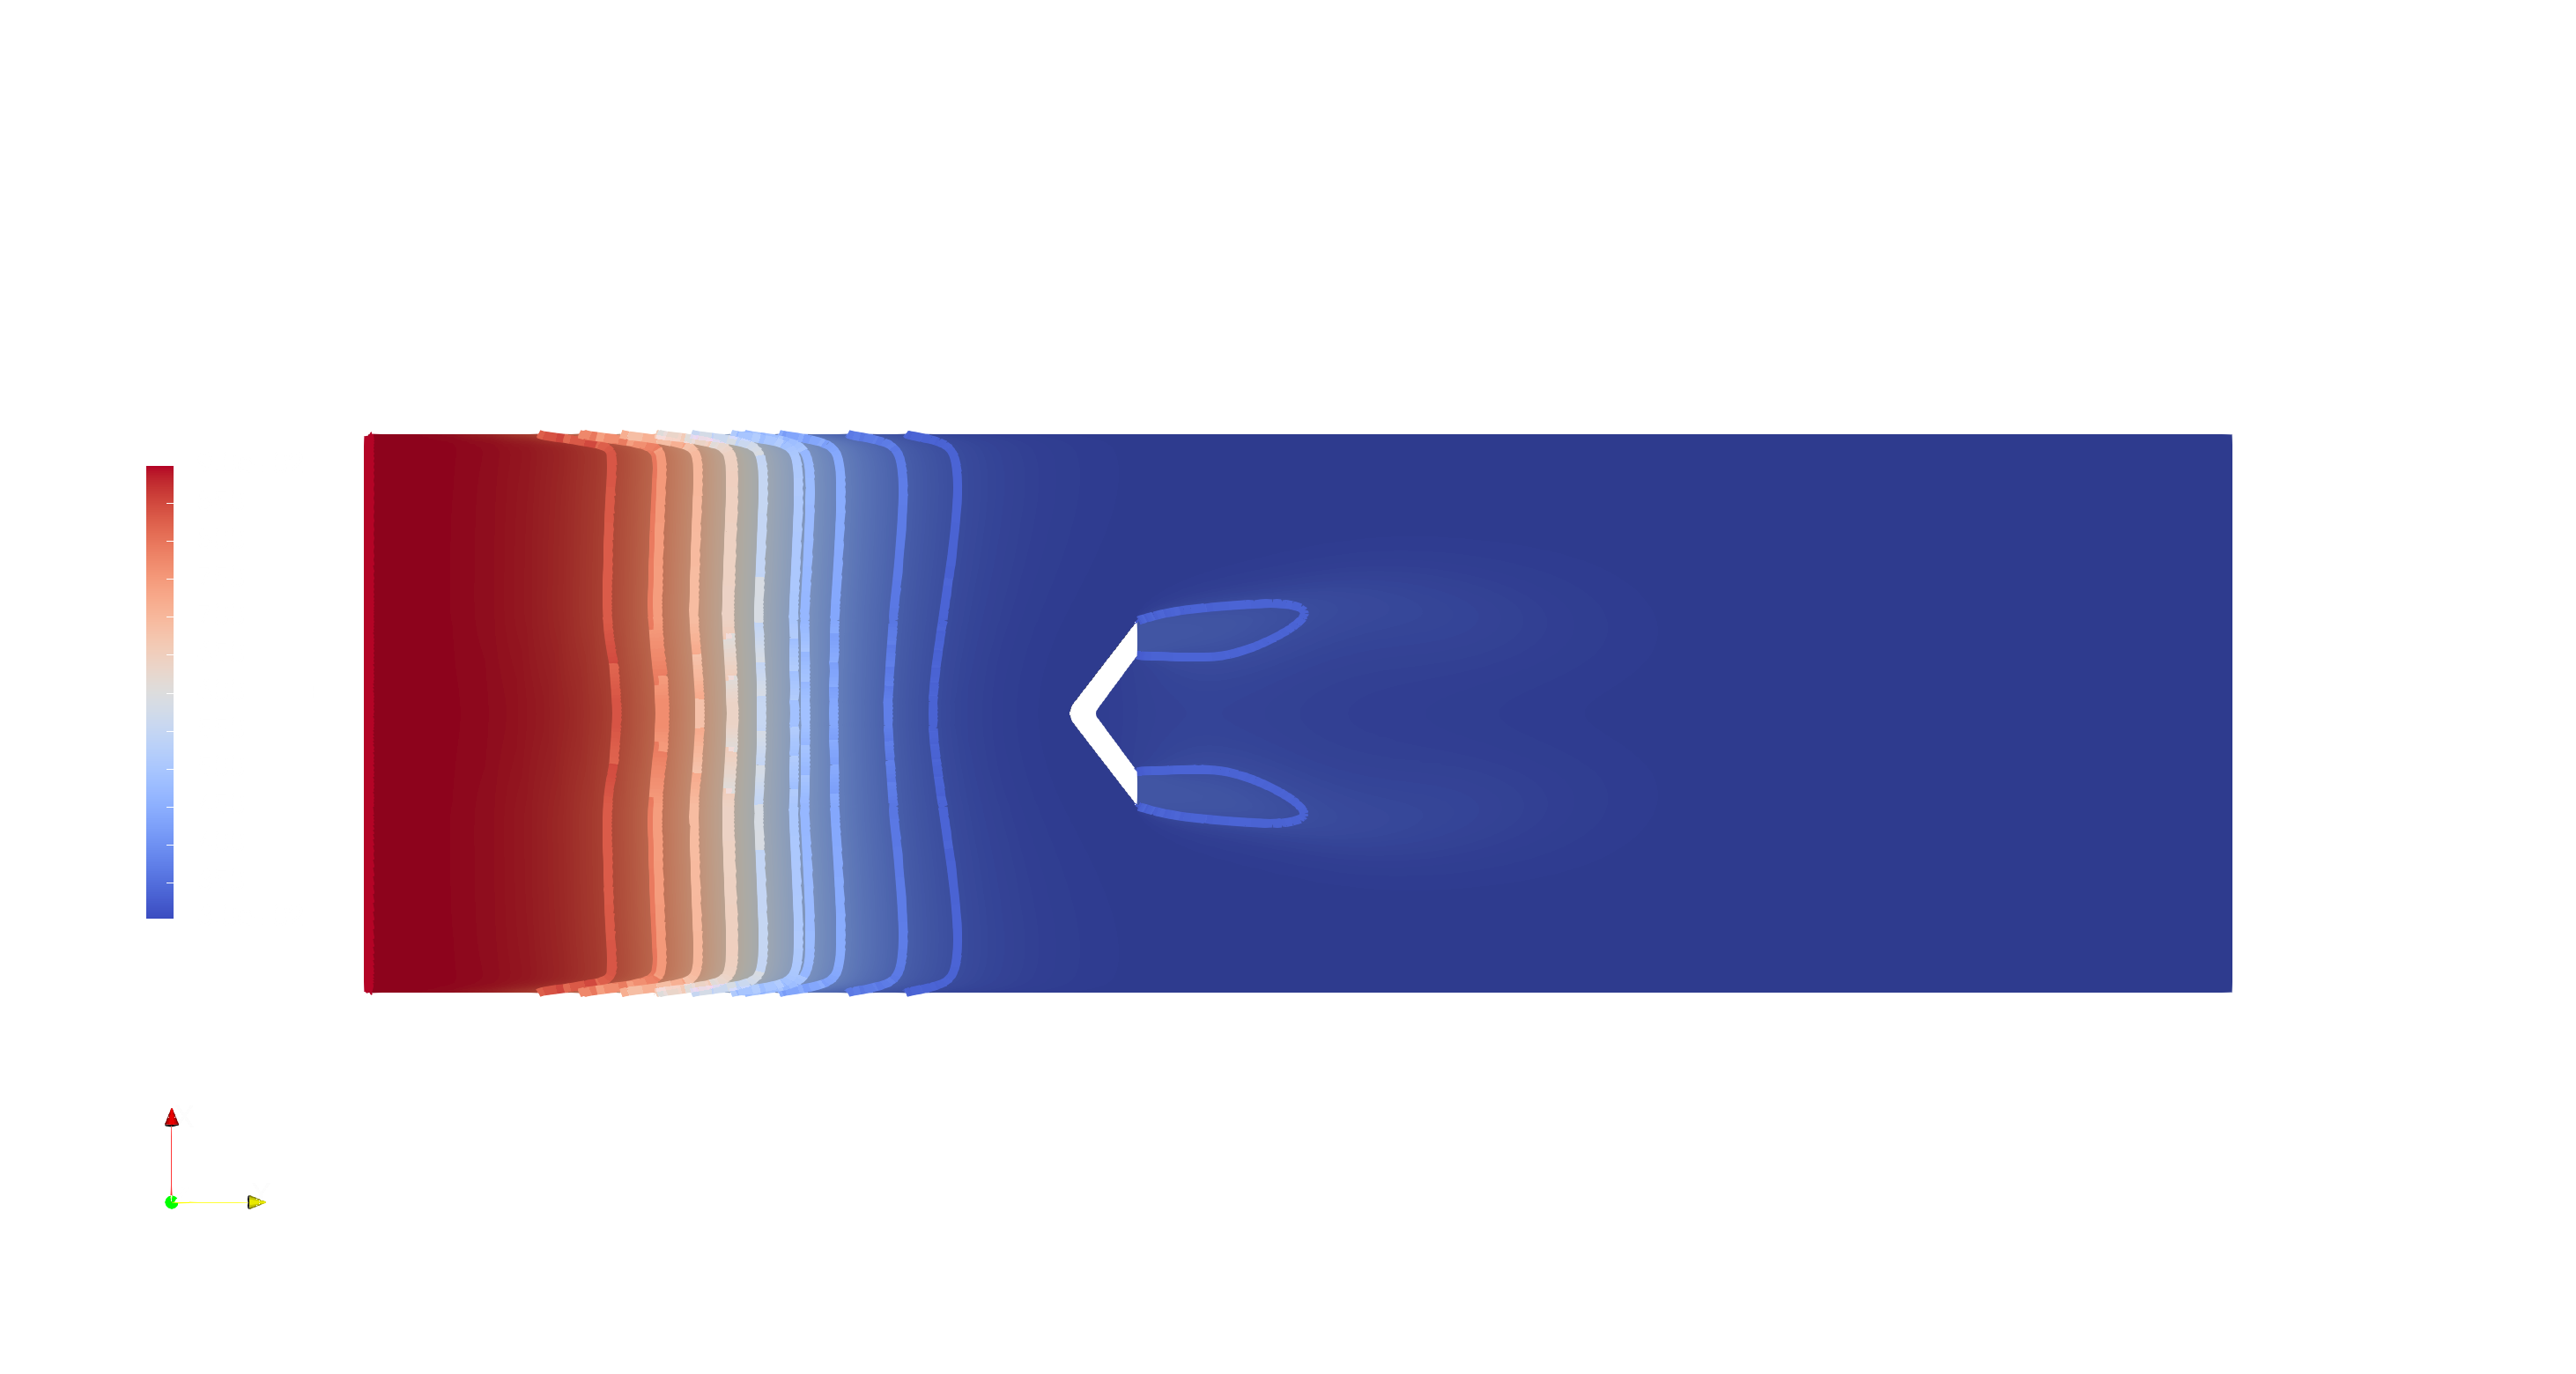
\includegraphics[height=0.25\textheight]{latexFIGS/figs/combustorT_002.png}
        \cprotect\caption{\verb|T| contour plot, $t = 0.02s$.}
    \end{figure}
    
    \begin{figure}[!h]
        \centering
        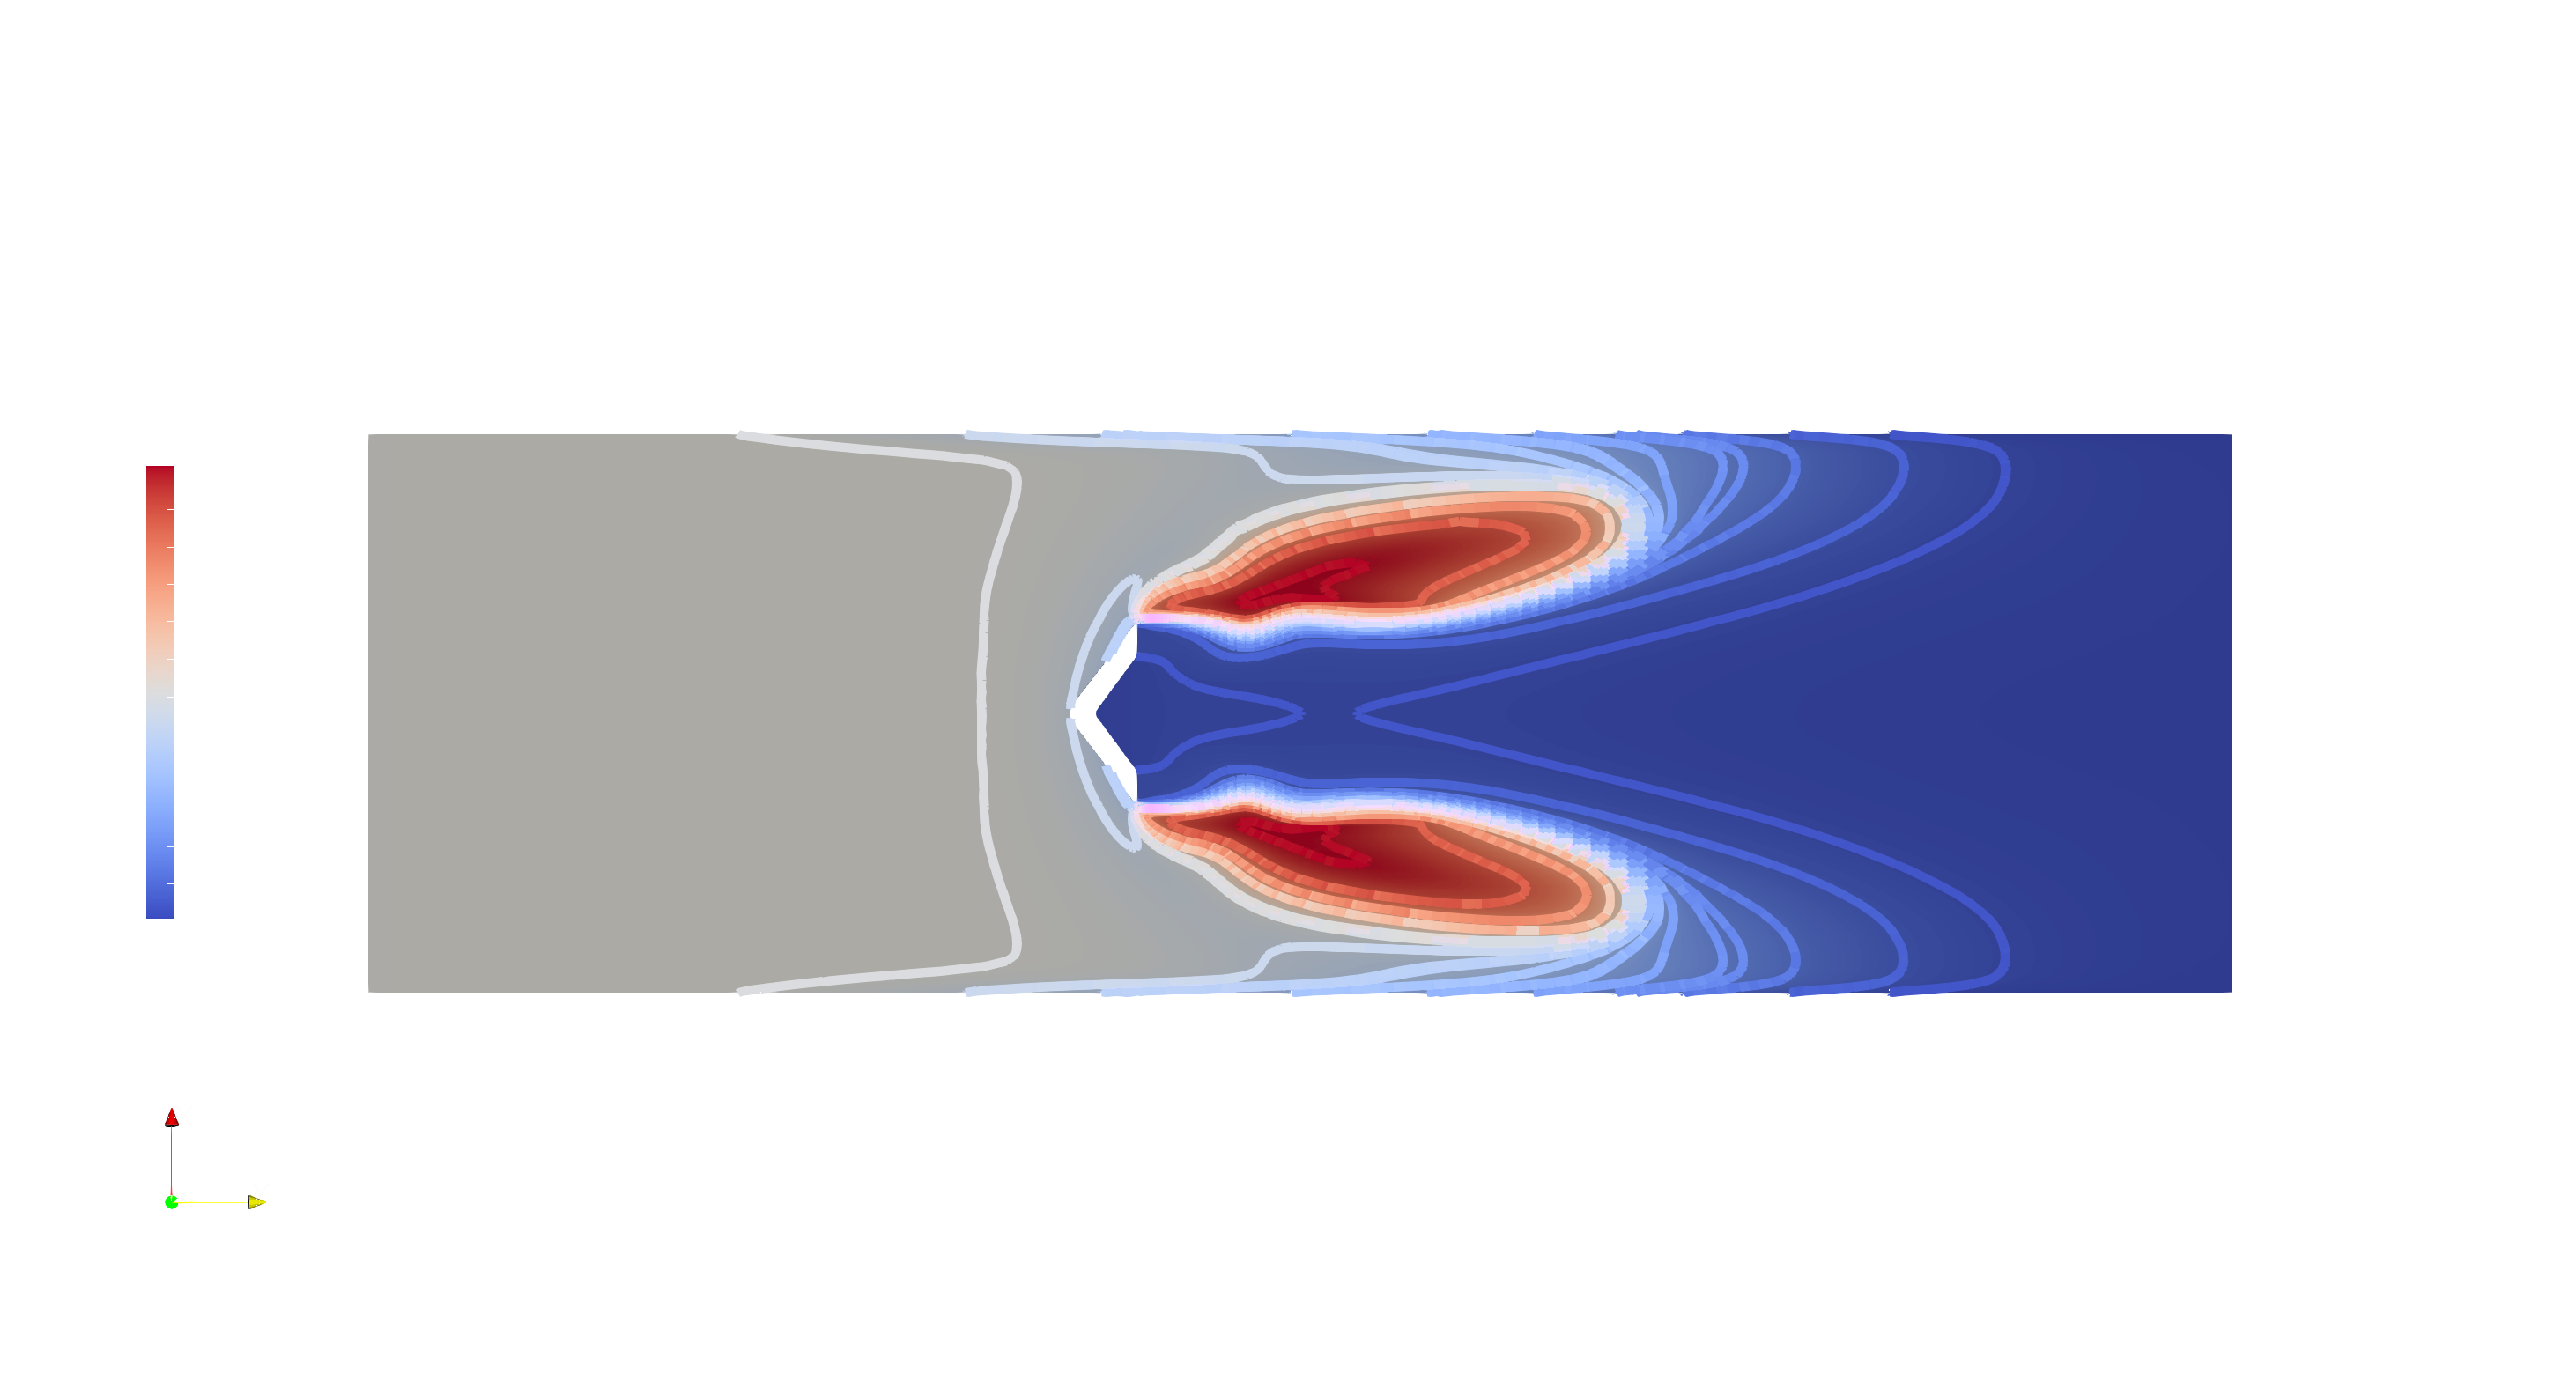
\includegraphics[height=0.25\textheight]{latexFIGS/figs/combustorT_005.png}
        \cprotect\caption{\verb|T| contour plot, $t = 0.05s$.}
    \end{figure}
    
    \begin{figure}[!hb]
        \centering
        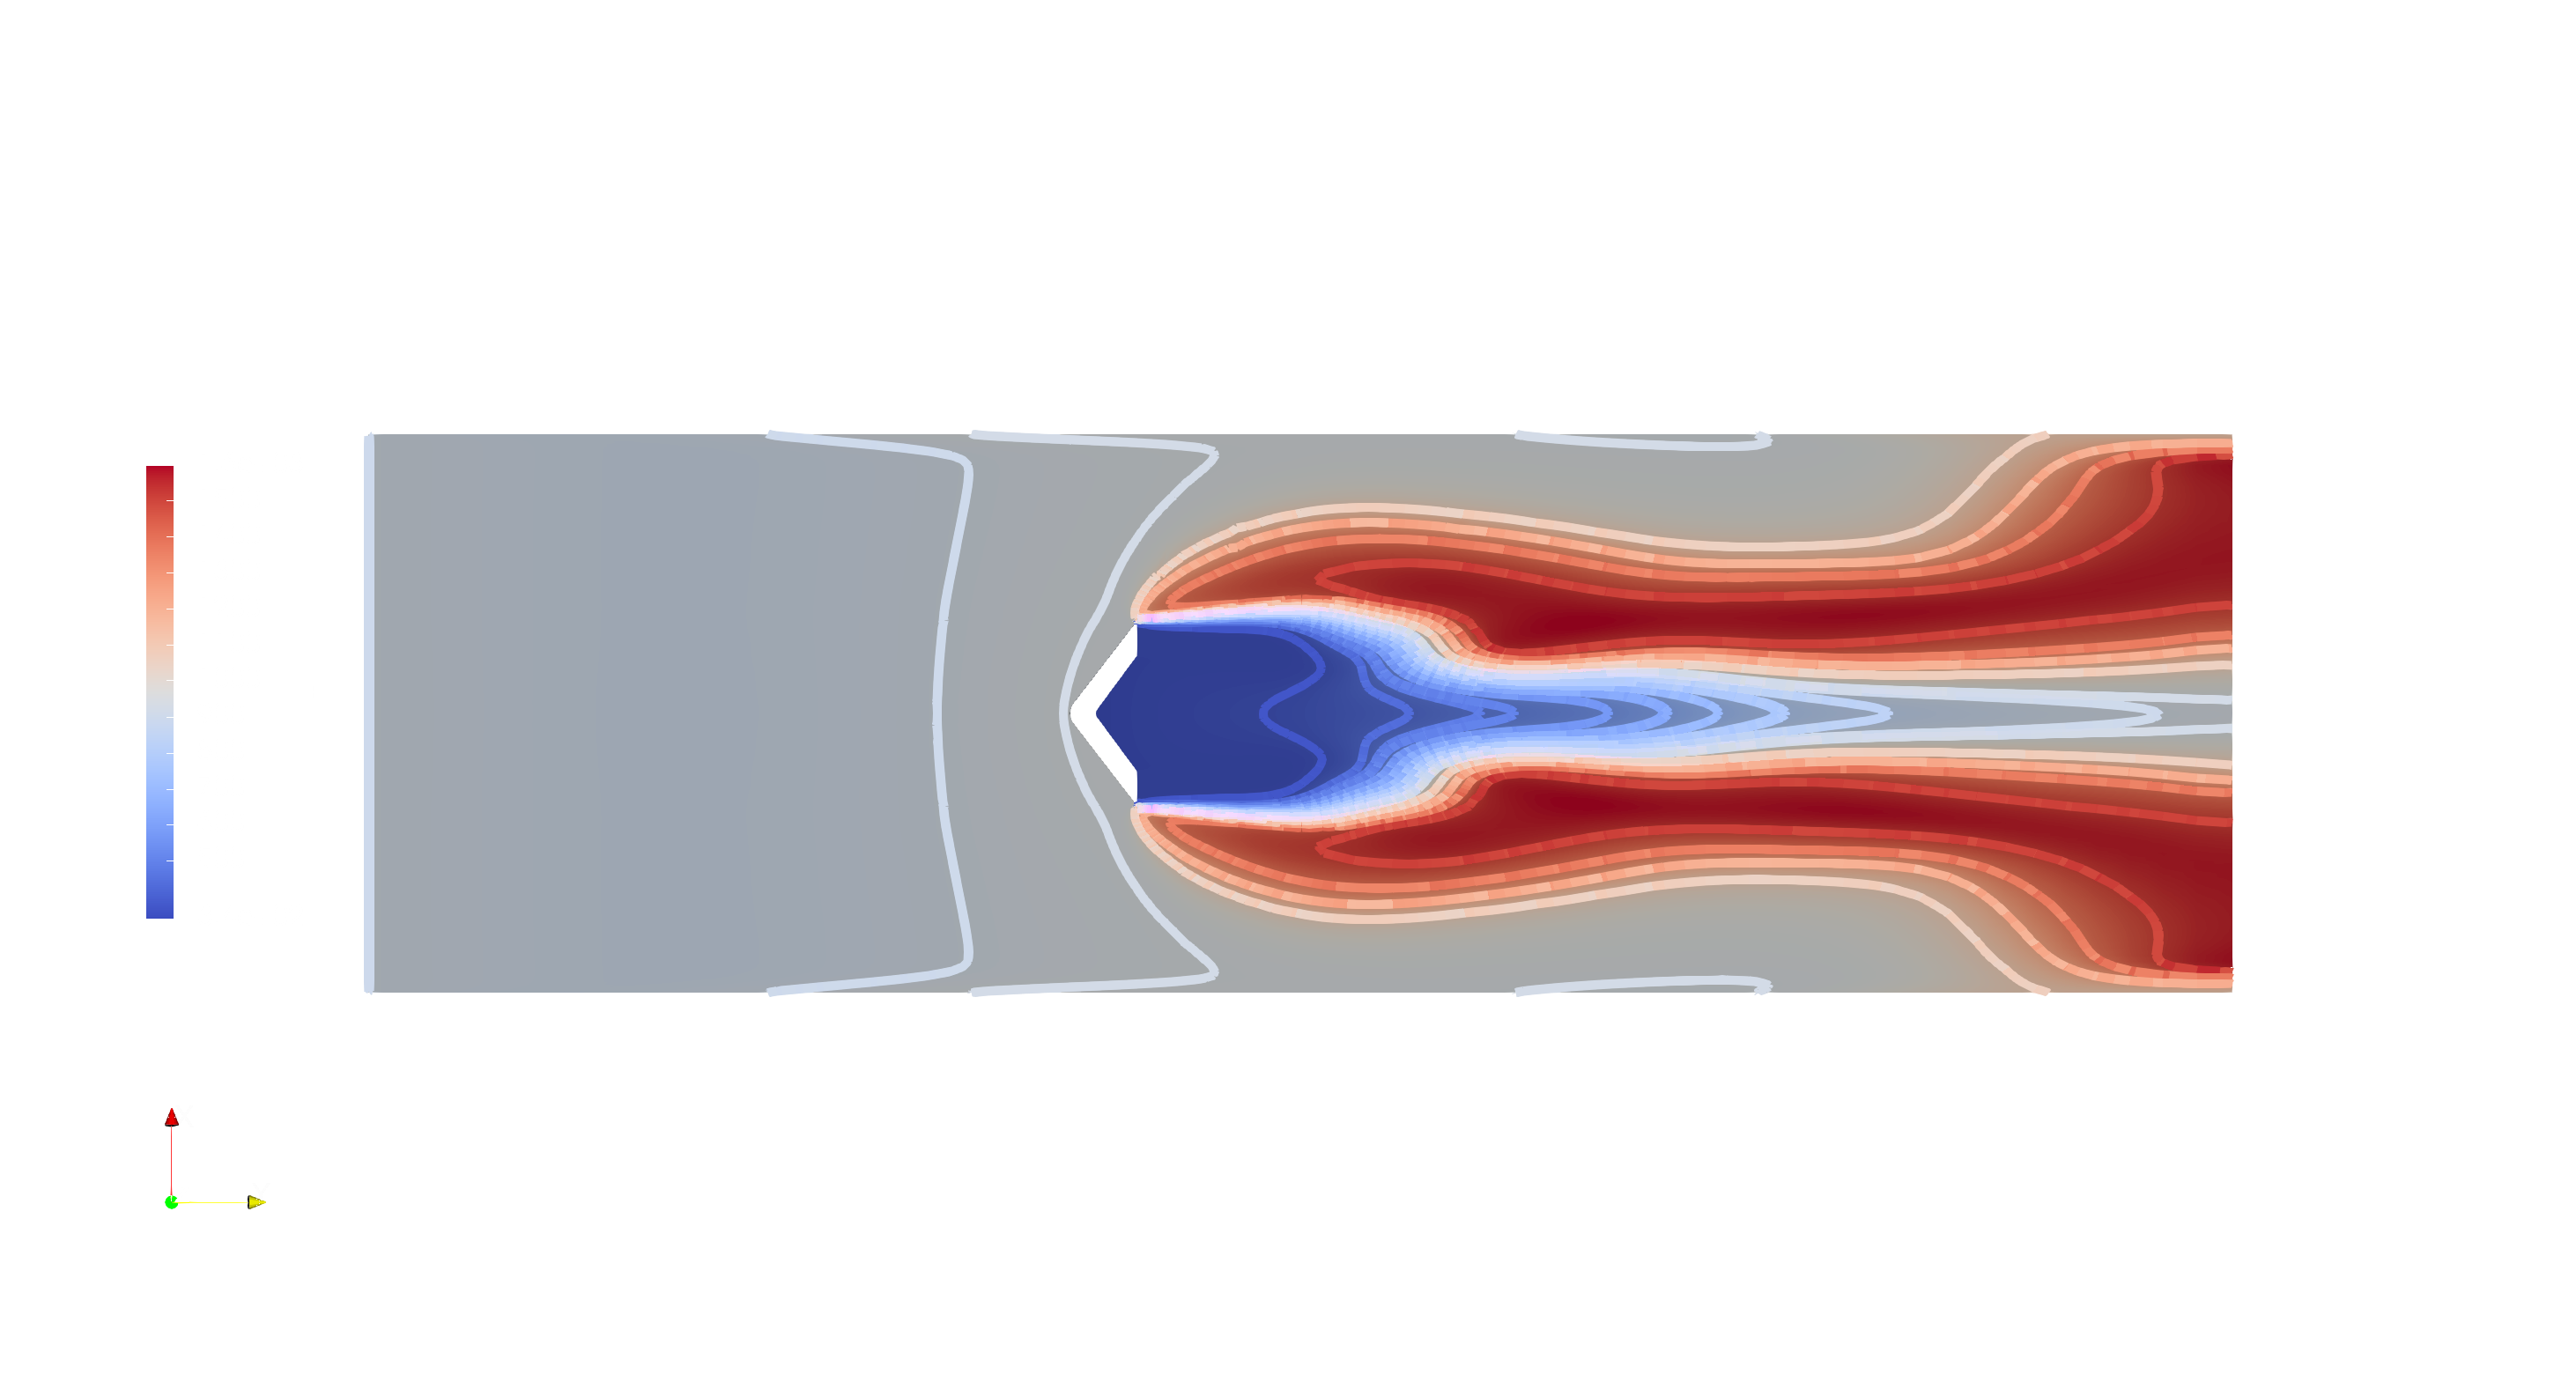
\includegraphics[height=0.25\textheight]{latexFIGS/figs/combustorT_008.png}
        \cprotect\caption{\verb|T| contour plot, $t = 0.08s$.}
    \end{figure}

    \begin{figure}[!ht]
        \centering
        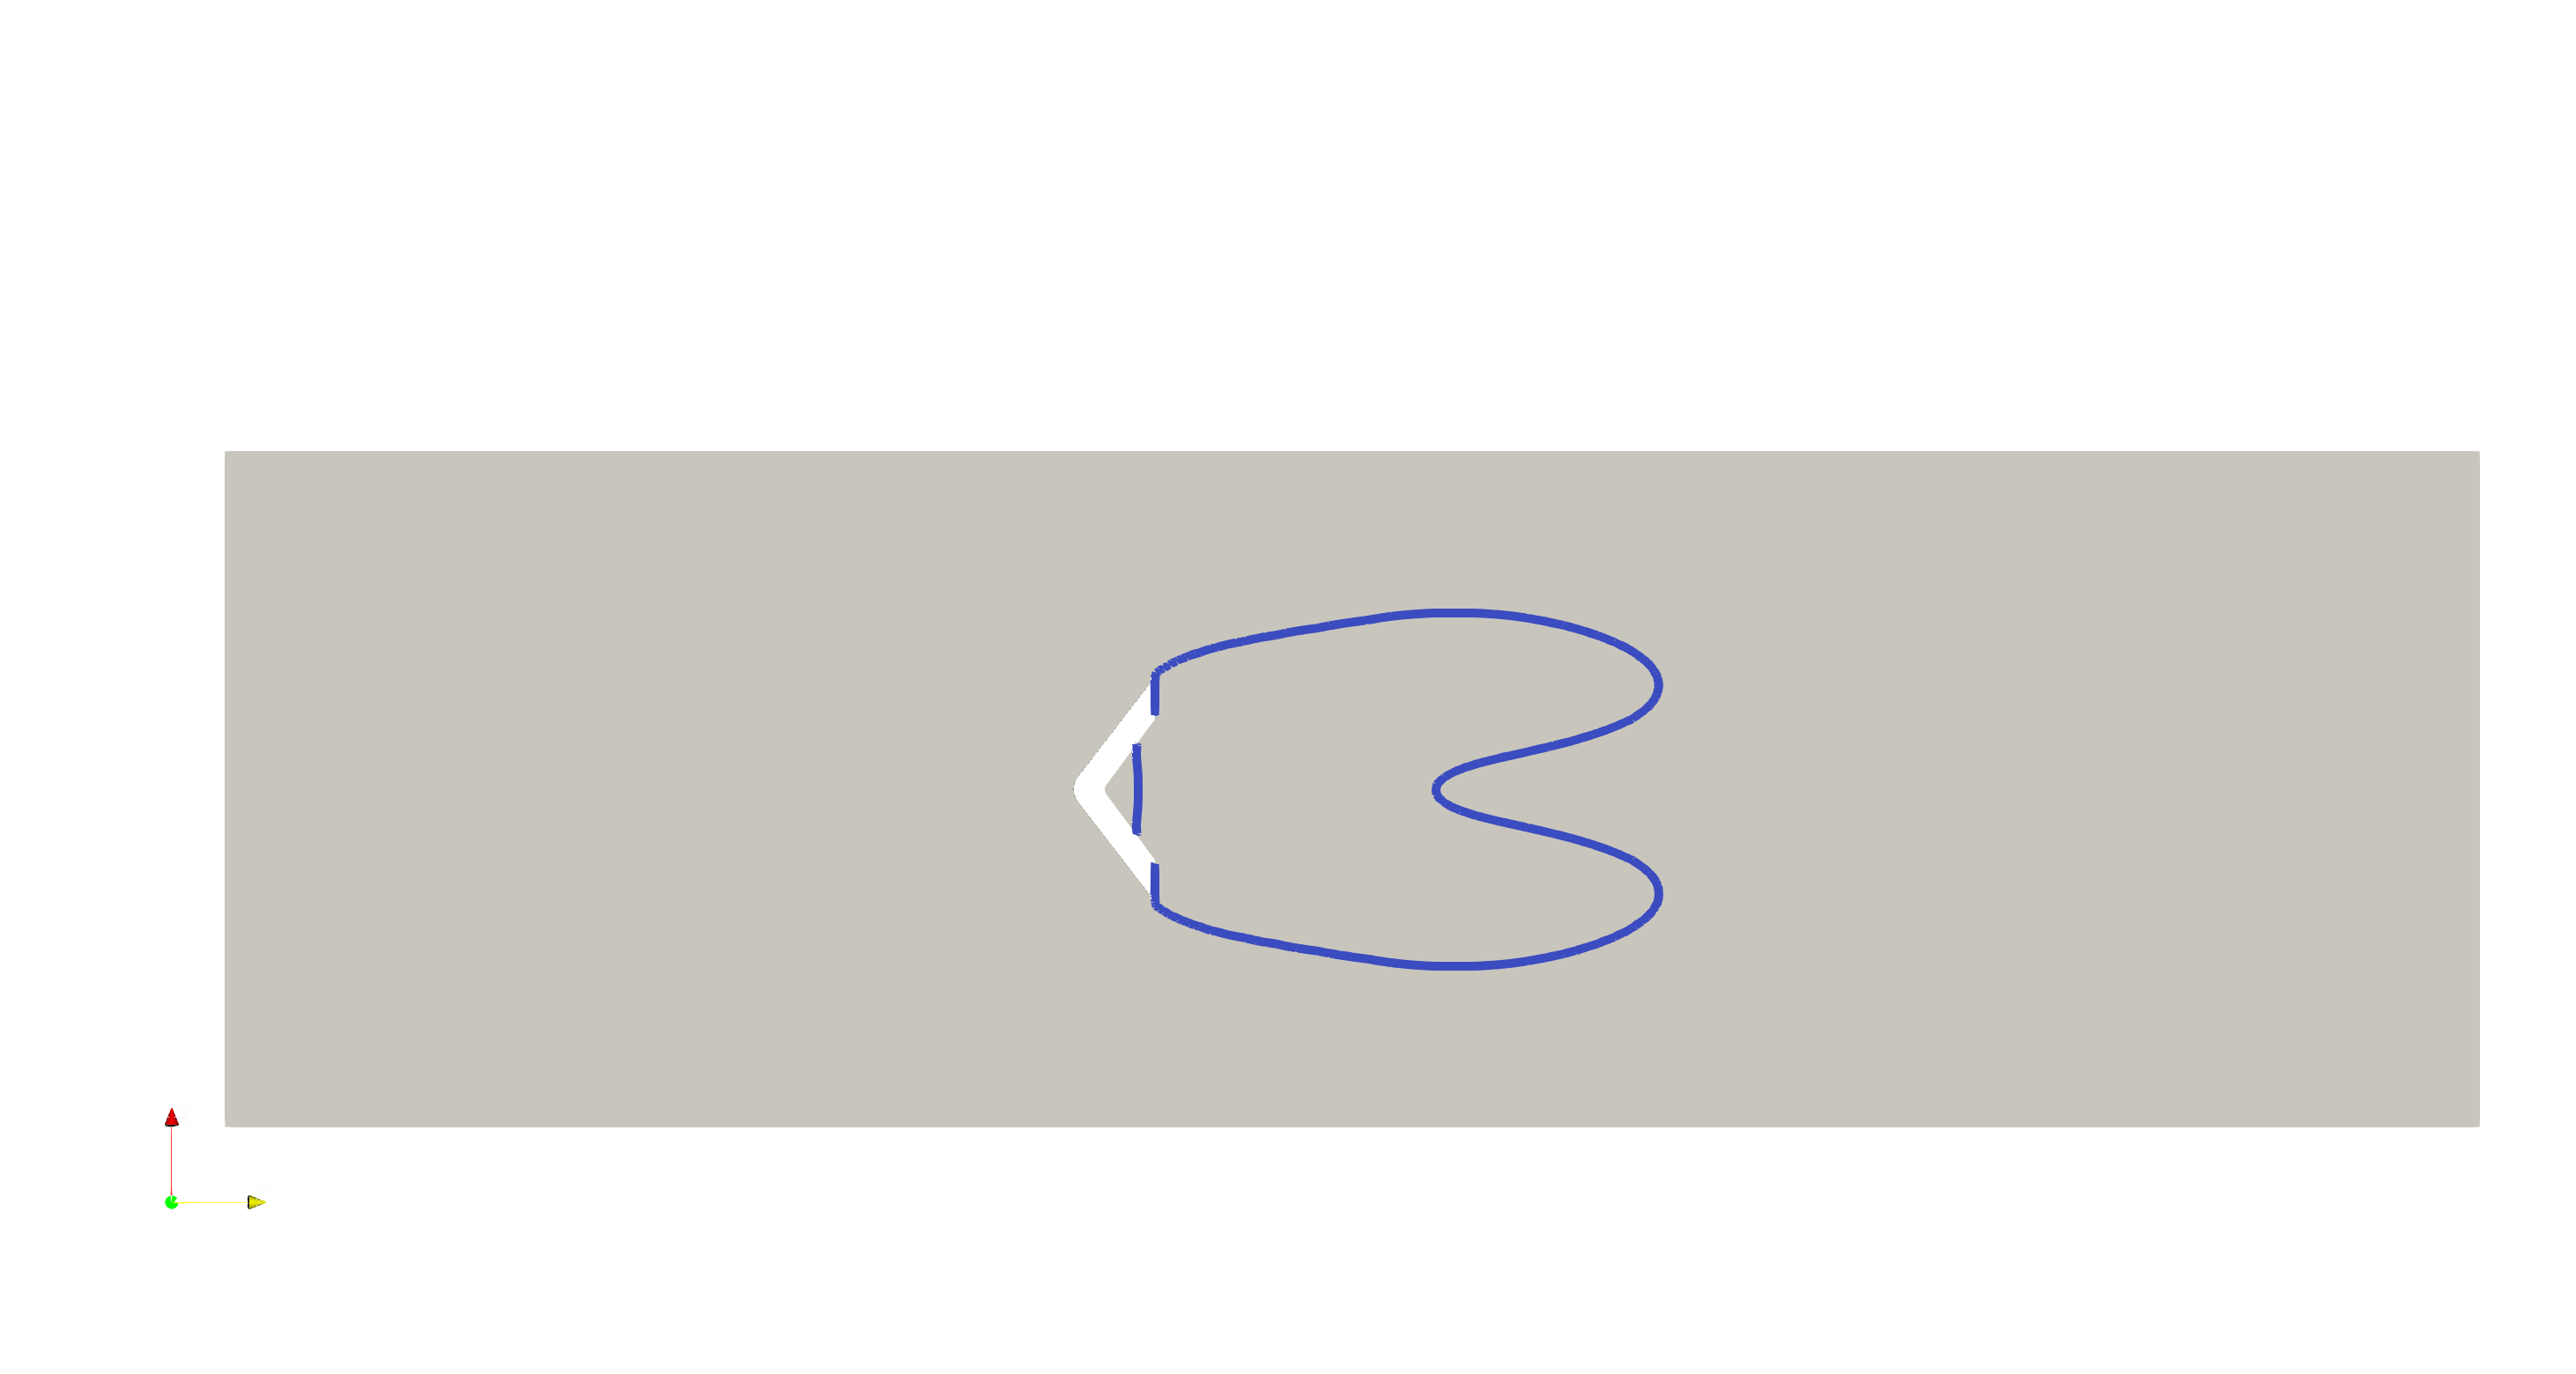
\includegraphics[height=0.25\textheight]{latexFIGS/figs/combustorSTOI1_002.png}
        \cprotect\caption{\verb|A/F| stoichiometric contour plot, $t = 0.02s$.}
    \end{figure}
    
    \begin{figure}[!h]
        \centering
        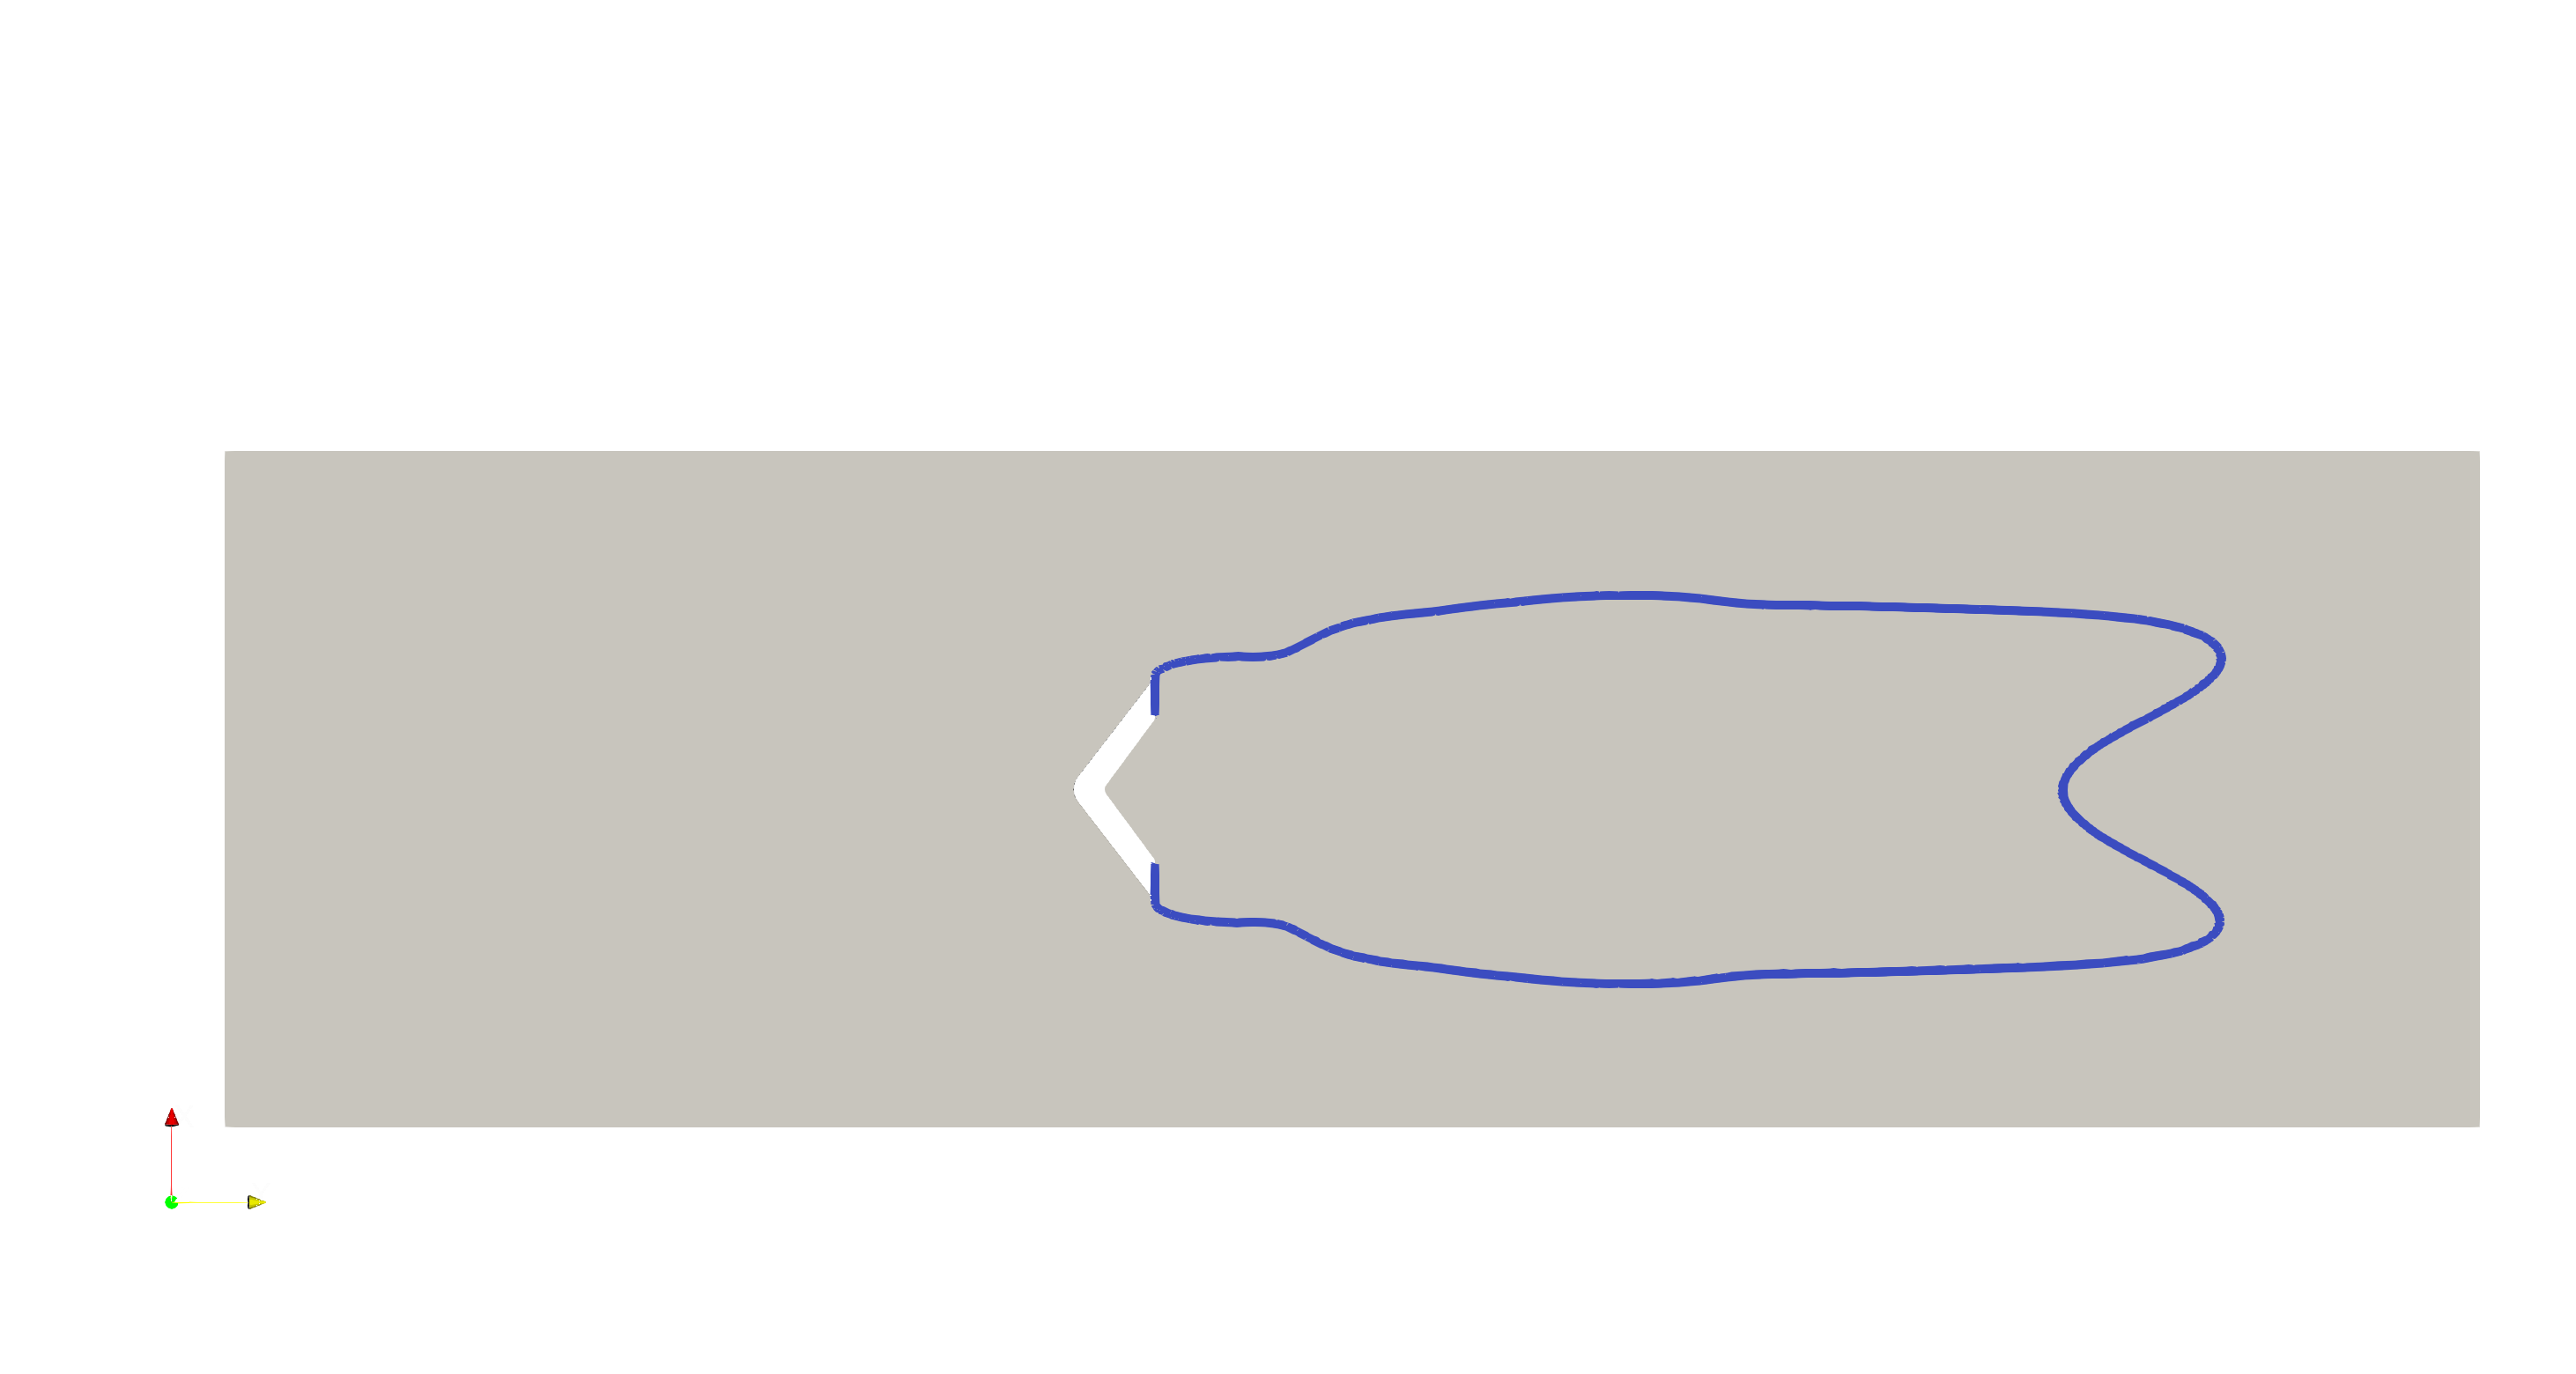
\includegraphics[height=0.25\textheight]{latexFIGS/figs/combustorSTOI1_005.png}
        \cprotect\caption{\verb|A/F| stoichiometric contour plot, $t = 0.05s$.}
    \end{figure}
    
    \begin{figure}[!hb]
        \centering
        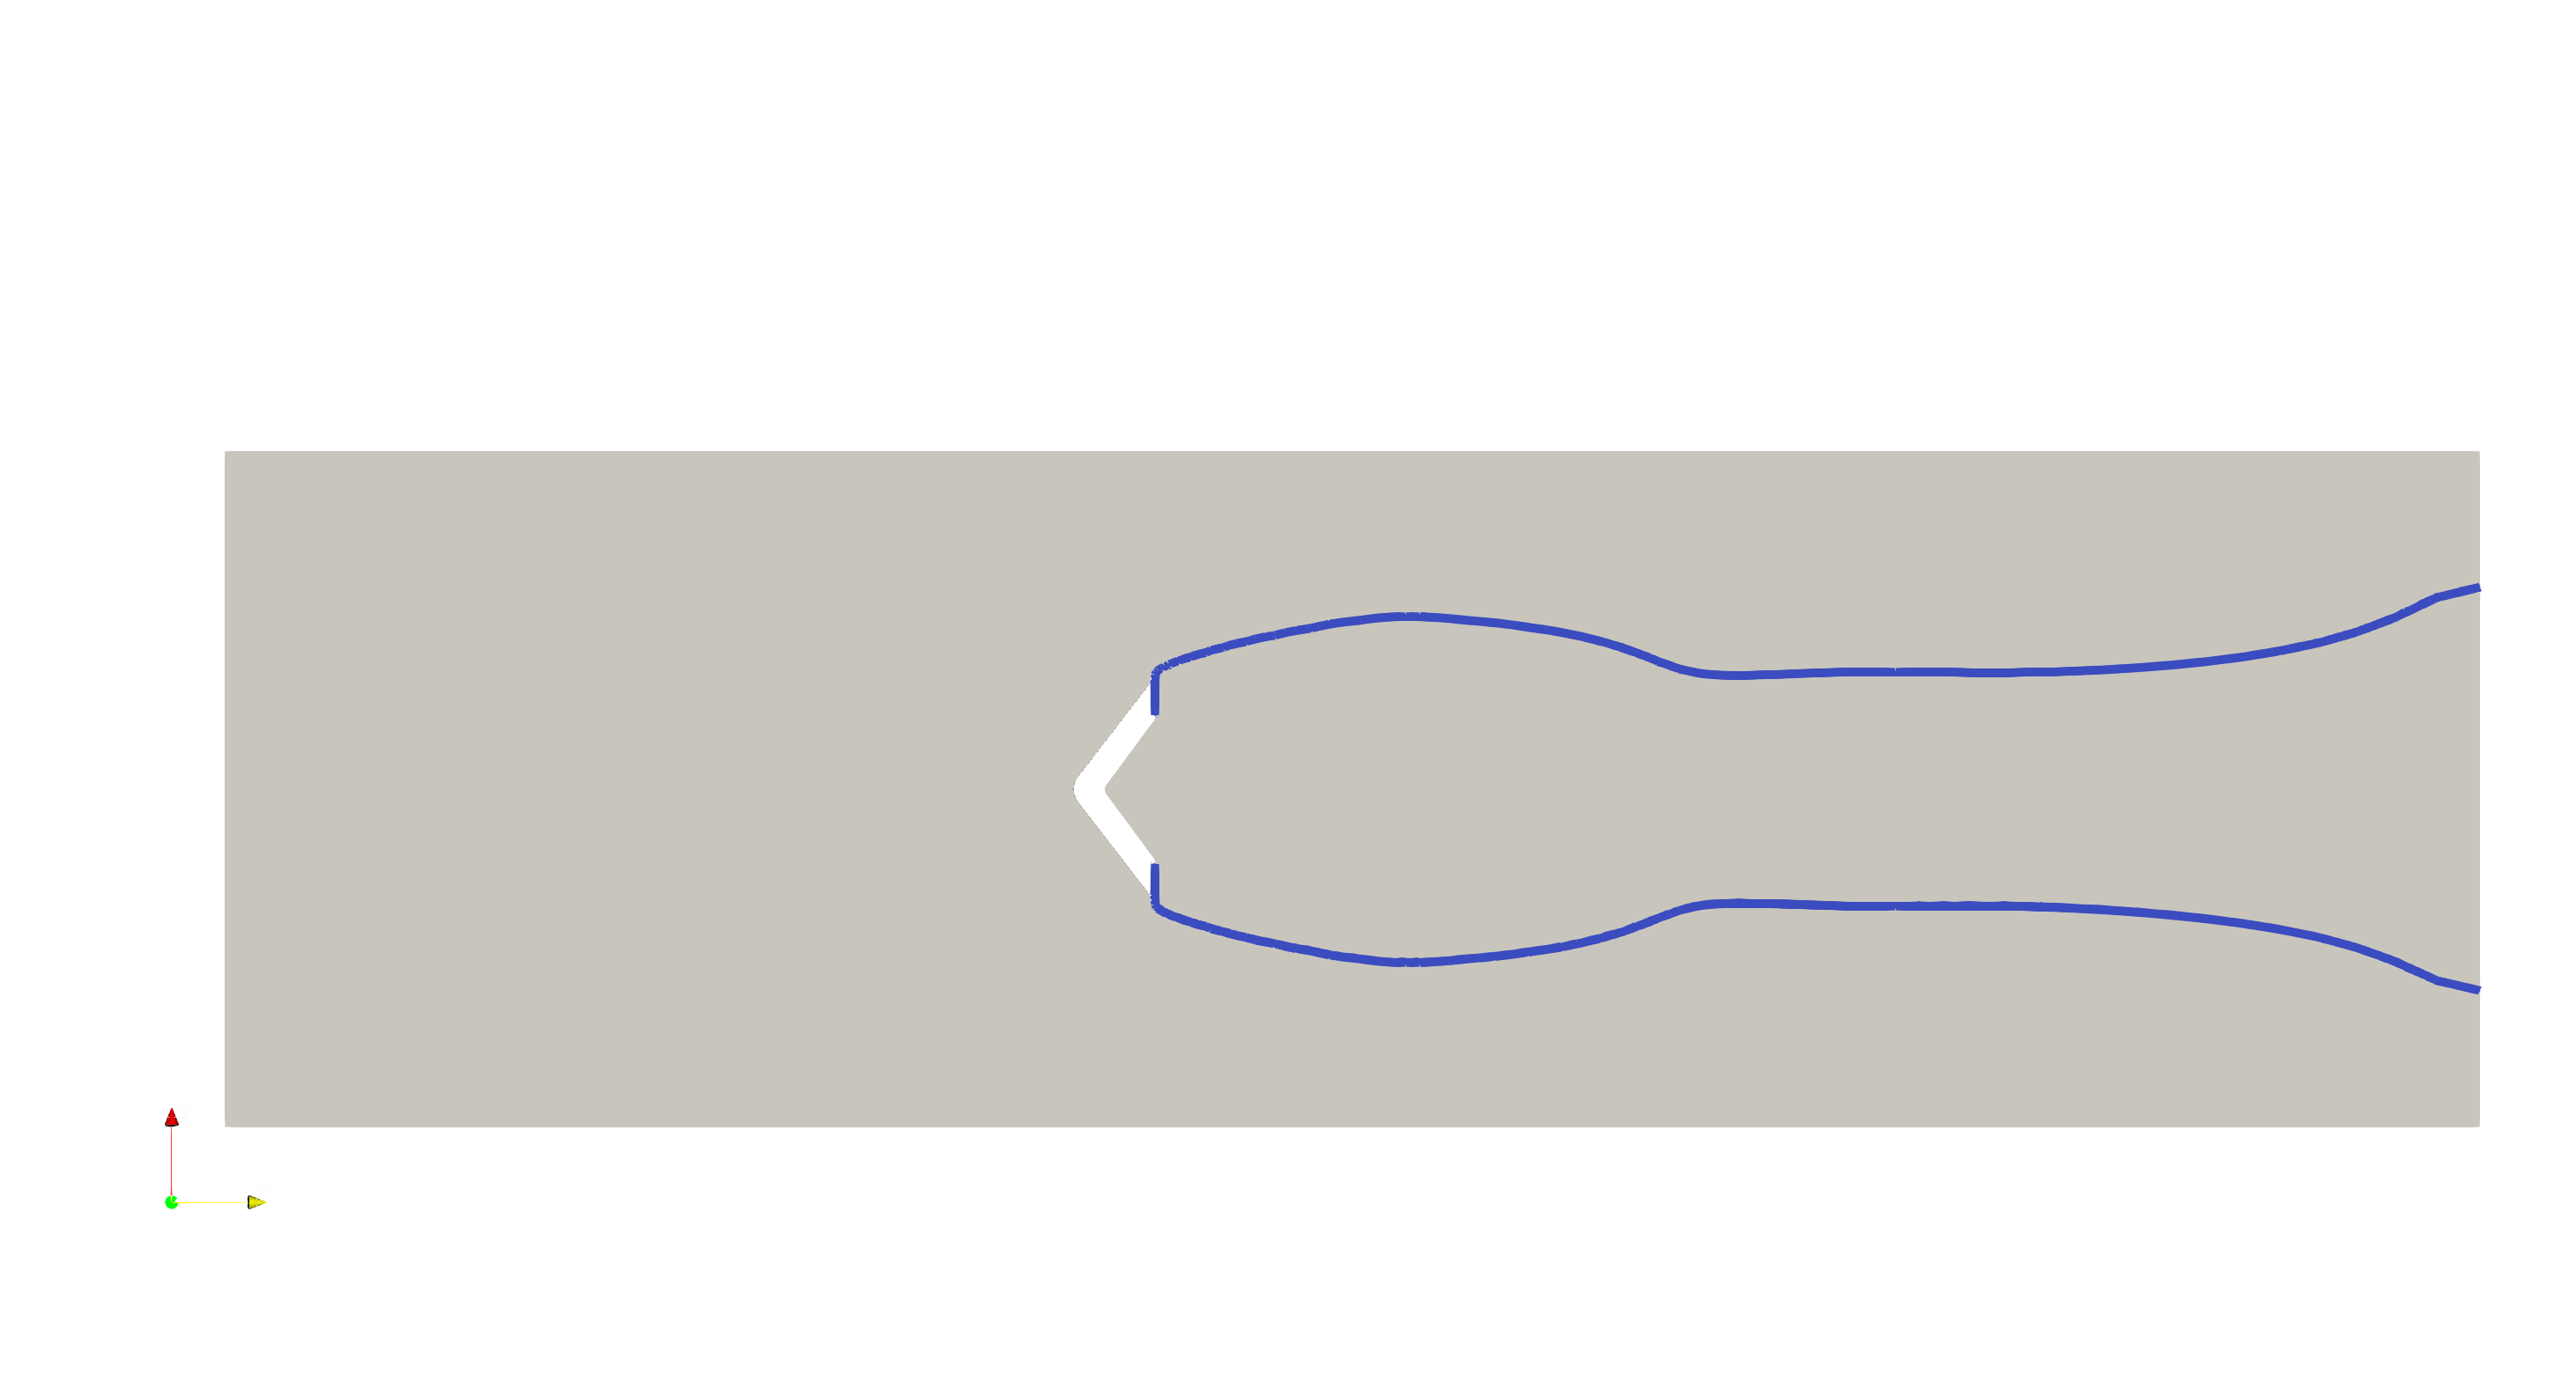
\includegraphics[height=0.25\textheight]{latexFIGS/figs/combustorSTOI1_008.png}
        \cprotect\caption{\verb|A/F| stoichimetric contour plot, $t = 0.08s$.}
    \end{figure}
    \clearpage
